The conveyor belt layer is managed by the PLC and is solely responsible for controlling the conveyor belts movement. This layer has one subsystem: The ON/OFF controller, which recieves signals from the PLC to start or stop the conveyor belt based on when the UR20 robot arm is ready to receive another box. The control of the conveyor belt is simplified to an ON/OFF mechanism, rather than dyanmically adjusting speed based on palletizing rate.

\begin{figure}[h!]
	\centering
 	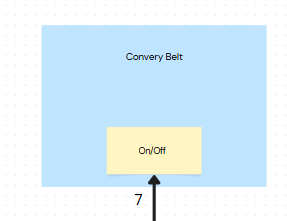
\includegraphics[width=0.60\textwidth]{images/convery_belt}
 \caption{Conveyor Belt Power Controller}
\end{figure}
\subsection{Power Controller Subsystem}
The power contoller subsystem in the conveyor belt layer is responsible for controlling the state of the conveyor belt. The subsystem receives a command from the PLC to switch the belt "ON" when the robot is prepared to recieve a new box and "OFF" once the box has been processed, ensuring smooth and controlled movement of boxes.
\subsubsection{Assumptions}
The assumption of a required automatic speed control is not required. The belts state change is assumed to be sufficient for the palletizing application, without the need to detect the exact positions of boxes on the belt. Only ensuring that the boxed move in a controlled manner when ready.

\subsubsection{Responsibilities}

The power controllers main responsibility is to maintain the stability of the conveyor, preventing any from advancing too far or falling off during the palletizing process. By managing the conveyor's ON/OFF state, it ensures that boxes are presented to the robot in a timely and safe manner. 

\subsubsection{Subsystem Interfaces}
The ON/OFF signal from the PLC serves as the sole input for the power controller. When the PLC sends an "ON" signal, the conveyor belt starts moving and will stop movement when the "OFF" signal is received. 

\begin {table}[H]
\caption {Controller Interface} 
\begin{center}
    \begin{tabular}{ | p{1cm} | p{6cm} | p{3cm} | p{3cm} |}
    \hline
    ID & Description & Inputs & Outputs \\ \hline
    \#16 & Power Controller signal & \pbox{3cm}{ ON/OFF } & \pbox{3cm}{NO OUTPUT}  \\ \hline
    \end{tabular}
\end{center}
\end{table}


